% Tema: bordas, set/reset, temporizadores (aula 06)
\question[6] A figura abaixo mostra o sinal de entrada \texttt{IN} de dois temporizadores ao longo do tempo, com o tempo programado \texttt{PT} indicado. Desenhe, nos espaços abaixo do sinal \texttt{IN}, a saída \texttt{Q} de um bloco \texttt{TON} e de um bloco \texttt{TOF}, ambos recebendo esse mesmo \texttt{IN} e o mesmo \texttt{PT}.

\begin{center}
\begin{tikzpicture}[scale=1]
  \draw[thick] (0,0) node[left] {IN} -- (1,0) -- (1,1) -- (4,1) -- (4,0) -- (8,0);
  \draw[dashed] (1,0) -- (1,-3.5);
  \draw[dashed] (2.5,0) -- (2.5,-3.5);
  \draw[dashed] (4,0) -- (4,-3.5);
  \draw[<->] (1,1.4) -- (2.5,1.4);
  \node[above] at (1.75,1.4) {PT};

  \node[left] at (0,-0.7) {Q (TON)};
  \draw[gray] (0,-1) -- (8,-1);

  \node[left] at (0,-2.7) {Q (TOF)};
  \draw[gray] (0,-3) -- (8,-3);

  \draw[->] (8,0) -- (8.3,0) node[right] {t};
\end{tikzpicture}
\end{center}

\begin{solution}
\begin{center}
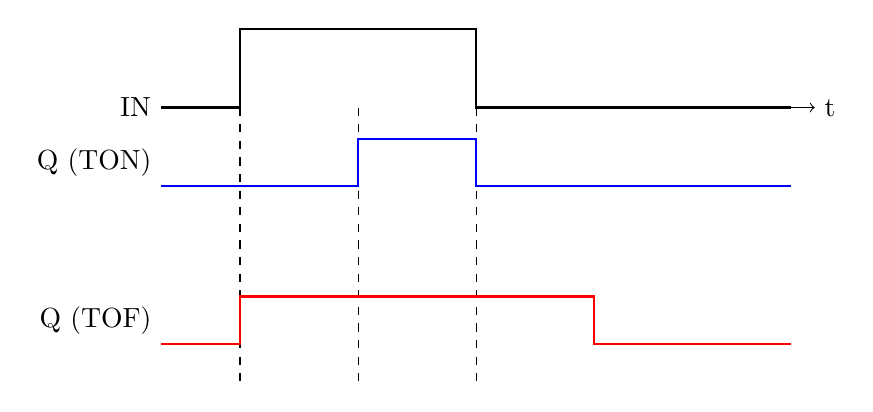
\begin{tikzpicture}[scale=1]
  \draw[thick] (0,0) node[left] {IN} -- (1,0) -- (1,1) -- (4,1) -- (4,0) -- (8,0);
  \draw[dashed] (1,0) -- (1,-3.5);
  \draw[dashed] (2.5,0) -- (2.5,-3.5);
  \draw[dashed] (4,0) -- (4,-3.5);

  \node[left] at (0,-0.7) {Q (TON)};
  \draw[thick, blue] (0,-1) -- (2.5,-1) -- (2.5,-0.4) -- (4,-0.4) -- (4,-1) -- (8,-1);

  \node[left] at (0,-2.7) {Q (TOF)};
  \draw[thick, red] (0,-3) -- (1,-3) -- (1,-2.4) -- (5.5,-2.4) -- (5.5,-3) -- (8,-3);

  \draw[->] (8,0) -- (8.3,0) node[right] {t};
\end{tikzpicture}
\end{center}
O \texttt{TON} atrasa a \textbf{subida} de \texttt{Q} em \texttt{PT} depois que \texttt{IN} sobe, e desce imediatamente quando \texttt{IN} cai. O \texttt{TOF} sobe imediatamente junto com \texttt{IN}, e atrasa a \textbf{descida} de \texttt{Q} em \texttt{PT} depois que \texttt{IN} cai.
\end{solution}
